%========== Divide & Conquer ==========%

\chapter{Divide \& Conquer}
\label{ch:divideandconquer}

\textbf{Relevant Assignment} Problem ?-?\\\\
\textbf{Pensum} CLRS Ch. 4 + 7 and SubCh. 2.3\\\\
\textbf{Algorithms} Merge sort, quicksort, fibonacci\\\\
\textbf{Keywords} Recurrences, master method
\vspace{1in}

\noindent Divide and conquer is a paradigm of algorithmic methodologies. It
takes a problem and \textit{divides} it into several smaller subproblems,
until it reaches a base case, which makes the algorithm \textit{bottom out},
or \textit{conquer} each of these subproblems. \textit{Combining} the
solutions of all of the subproblems then yields a correct solution to the
original problem.
\\\\
\noindent \textbf{Divide} the problem into a number of subproblems that are
smaller instances of the same problem.
\\\\
\noindent \textbf{Conquer} the subproblems by solving them recursively. If the
subproblem sizes are small enough, however, just solve the subproblems
trivially.
\\\\
\noindent \textbf{Combine} the solutions to the subproblems into the solution
for the original problem.
\\\\

\section{Solving Recurrences}
% p. 83-97, CLRS 
Divide and conquer algorithms give rise to recurrence naturally, because they
call themselves recursively. To analyze the complexity of any recursive
algorithm we must describe it mathematically as an equation or inequality.
\\\\
We do this using one of three methods.
\begin{description}
	\item \textbf{Recursion trees} describes the recursions by means of a
tree-structure, by which we can then either guess or argue the complexity.
	\item \textbf{Substitution} uses a guessed bound, which could have been
derived from a recursion tree, and then by mathematical induction proves this
bound.
	\item \textbf{Master method} provides formulae for recurrences of the form
$T(n) = a T(n/b) + f(n)$, where $a \geq 1$, $b > 1$ and $f(n)$ is a given
function.
\end{description}

\subsection{Recursion Trees}
% p. 88-92, CLRS
A recursion tree is a pictorial representation of an algorithms recursive
calls. That is, we simply draw the recursions as they occur in a
tree-structure, such that we may make a guess as to the complexity of an
algorithm.

\begin{figure}[h]
	\center
	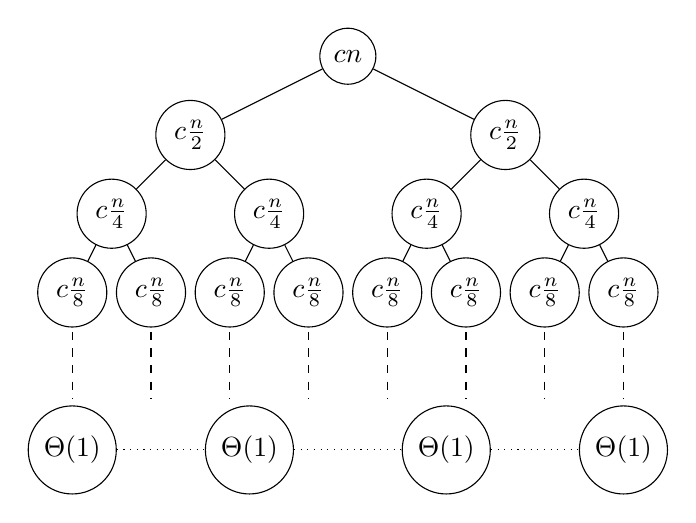
\begin{tikzpicture}
	[
	scale=1.0,
	align=center,
	every node/.style={circle, fill=white, draw=black}
	]
		% level 1
		\node (n1) at 	(3.5, -1) {$cn$};
		
		% level 2
		\node (n2) at 	(1.5, -2) {$c\frac{n}{2}$};
		\node (n3) at 	(5.5, -2) {$c\frac{n}{2}$};
		
		% level 3
		\node (n4) at 	(0.5, -3) {$c\frac{n}{4}$};
		\node (n5) at 	(2.5, -3) {$c\frac{n}{4}$};
		\node (n6) at 	(4.5, -3) {$c\frac{n}{4}$};
		\node (n7) at 	(6.5, -3) {$c\frac{n}{4}$};
		
		% level 4
		\node (n8) at 	(0, -4) {$c\frac{n}{8}$};
		\node (n9) at 	(1, -4) {$c\frac{n}{8}$};
		\node (n10) at 	(2, -4) {$c\frac{n}{8}$};
		\node (n11) at 	(3, -4) {$c\frac{n}{8}$};
		\node (n12) at 	(4, -4) {$c\frac{n}{8}$};
		\node (n13) at 	(5, -4) {$c\frac{n}{8}$};
		\node (n14) at 	(6, -4) {$c\frac{n}{8}$};
		\node (n15) at 	(7, -4) {$c\frac{n}{8}$};
		
		% bottom-out level
		\node (l1) at (0, -6) {$\Theta(1)$};
		\node (l2) at (2.25, -6) {$\Theta(1)$};
		\node (l3) at (4.75, -6) {$\Theta(1)$};
		\node (l4) at (7, -6) {$\Theta(1)$};
		
		% drawing code
		\draw [dashed] (0, -4.5) -- (0, -5.35);
		\draw [dashed] (1, -4.5) -- (1, -5.35);
		\draw [dashed] (2, -4.5) -- (2, -5.35);
		\draw [dashed] (3, -4.5) -- (3, -5.35);
		\draw [dashed] (4, -4.5) -- (4, -5.35);
		\draw [dashed] (5, -4.5) -- (5, -5.35);
		\draw [dashed] (6, -4.5) -- (6, -5.35);
		\draw [dashed] (7, -4.5) -- (7, -5.35);
		\foreach \from/\to in {n1/n2,n1/n3} \draw (\from) -- (\to);
		\foreach \from/\to in {n2/n4,n2/n5,n3/n6,n3/n7} \draw (\from) -- (\to);
		\foreach \from/\to in {n4/n8,n4/n9,n5/n10,n5/n11,n6/n12,n6/n13,n7/n14,n7/n15} \draw (\from) -- (\to);
		\foreach \from/\to in {l1/l2,l2/l3,l3/l4} \draw [dotted] (\from) -- (\to);
	\end{tikzpicture}

	\caption{Recurrence tree of merge sort.}
\end{figure}

Although recursion trees are useful for getting an idea about the complexity
of a recursive algorithm, it doesn't directly give us any concrete about this.
For that must employ more strict methods that are rooted in mathematics, and
not drawings - we can do this by induction with the substitution method (see
section \ref{ch:divideandconquer|sub:recurrences|subsub:substitution}).

\subsection{Substitution}
\label{ch:divideandconquer|sub:recurrences|subsub:substitution}
% p. 83-87, CLRS
The substitution method for solving recurrences consists of
two steps:
\begin{itemize}
\item Guess the form of the solution.
\item Use mathematical induction to find constants in the form and show that
the solution works.
\end{itemize}
The inductive hypothesis is applied to smaller values,
similar like recursive calls bring us closer to the base case
\\\\
\noindent \textbf{Example}\\
The recurrence relation for the cost of a divide-and-conquer method is
$T(n) = 2T( \lfloor n/2 \rfloor ) + n$. Our induction hypothesis of $T(n)$ is
$O(n \lg n)$ or $T(n) \leq cn \lg n$ for some constant $c$, independent of $n$.

Assume the hypothesis holds for all $m < n$ and substitute:
\begin{align}
	T(n) &\leq 2(c \lfloor n/2 \rfloor \lg_2 (\lfloor n/2 \rfloor )) + n \\
	&\leq cn \lg_2(n/2)+n \\
	&= cn \lg_2(n) - cn \lg_2(2)+n \\
	&= cn \lg_2(n) - cn + n \\
	&\leq cn \lg_2 (n)
\end{align}
as long as $c \geq 1$.

\newpage
\subsection{The Master Method}
% p. 88-97, CLRS
For a divide-and-conquer algorithm $T(n)$, let $a$ denote the number of
subproblems created, and $n/b$ denote the size of each of these, on each
recursion. For each recursion we have a combine step, which takes $f(n)$.
We then have a recurrence of the form $T(n) = a T(n/b) + f(n)$.

Algorithms of this form can be solved by means of the master theorem, which
is given by
\begin{align}
	T(n) &= a T\left(\frac{n}{b}\right) + f(n)
	\begin{cases}
		f(n) = O(n^{\lg_b a - \epsilon}) & T(n) = \Theta(n^{\lg_b a}) \\
		f(n) = \Theta(n^{\lg_b a}) & T(n) = \Theta(n^{\lg_b a} \lg n) \\
		f(n) = O(n^{\lg_b a + \epsilon}) & * \Rightarrow T(n) = \Theta(f(n))
	\end{cases}
\end{align}
where $a \geq 1$, $b > 1$ and $\epsilon > 0$.
\begin{align}
	a f\left(\frac{n}{b}\right) &\leq c f(n)
	\text{, for all sufficiently large } n \text{, where } c < 1 \tag{*}
\end{align}
The first case $O(n^{\lg_b a - \epsilon})$ occurs when the \textit{divide}
step of the algorithm contributes the most to the complexity of the algorithm,
since $n^{\lg_b a} > f(n)$, and we therefore have to account for this by
subtracting $\epsilon$ from the exponent on the left-hand side. Vice versa for
the third case $O(n^{\lg_b a + \epsilon})$, which is symmetric. The second
case $\Theta(n^{\lg_b a})$ occurs when both steps, the \textit{divide} and
\textit{combine} step, are of the same complexity.
\\\\
\noindent \textbf{Example} \\
Consider the recurrence $T(n) = 2T(n/2) + f(n)$ of merge sort. We identify the
variables values as $a = 2$ since each recursive call creates two subproblems
and $b = 2$ since each of these are of $n/2$ the size of the previous problem.
The combine step is of linear time $\Theta(n)$.

We then have that $O(n^{\lg_2 2}) = f(n)$, since $f(n) = \Theta(n)$ and this
satisfies the previous equation, because $O(n^{\lg_2 2}) = \Theta(n)$.
Therefore, the second case of the master theorem applies to this algorithm,
and the complexity of it is then $\Theta(n^{lg_2 2}\lg n) = \Theta(n \lg n)$.




